\documentclass{article}

% Useful packages
\usepackage[dutch]{babel} % Nederlands taalpakket
\usepackage{multicol}
\setlength{\columnsep}{1cm}

% Set page size and margins
% Replace `letterpaper' with `a4paper' for UK/EU standard size
\usepackage[a4paper,top=2cm,bottom=2cm,left=2cm,right=2cm,marginparwidth=1.75cm]{geometry}

\usepackage{caption}
\usepackage{amsmath}
\usepackage{siunitx}
\usepackage{wrapfig}
\usepackage{float}
\usepackage{graphicx}
\graphicspath{{images/}}
\usepackage{subcaption}
\usepackage[colorlinks=true, allcolors=blue]{hyperref}
\usepackage{xcolor}
\usepackage{listings}
\usepackage{import}
\usepackage{xcolor}
\usepackage[toc,page]{appendix} % Pakket voor het maken van bijlagen
\usepackage{hyperref} % Pakket voor hyperlinks en verwijzingen
\usepackage{rotating}
\usepackage{array}
\usepackage{lscape}


% Definieer de kleuren voor syntax highlighting
\definecolor{codegreen}{rgb}{0,0.6,0}
\definecolor{codegray}{rgb}{0.5,0.5,0.5}
\definecolor{codepurple}{rgb}{0.58,0,0.82}
\definecolor{backcolour}{rgb}{0.95,0.95,0.92}

\lstdefinestyle{mystyle}{
    backgroundcolor=\color{backcolour},
    commentstyle=\color{codegreen},
    keywordstyle=\color{codepurple},
    numberstyle=\tiny\color{codegray},
    basicstyle=\footnotesize\ttfamily,
    breakatwhitespace=false,
    breaklines=true,
    captionpos=b,
    keepspaces=true,
    numbers=left,
    numbersep=5pt,
    showspaces=false,
    showstringspaces=false,
    showtabs=false,
    tabsize=2
}

\usepackage[dutch]{babel}% Language setting


\title{
    Life Cycle Engineering \\
    \large Uitvoeren van safety/reliability analyse}

\author{
  Vollmuller, Michel\\
  1809572\\
  \texttt{michel.vollmuller@student.hu.nl}
} 

\begin{document}
\maketitle

% \begin{abstract}
%   Dit onderzoek richt zich op de aandrijftechniek van een moonrover gebaseerd op een iris, waarbij verschillende aspecten worden geanalyseerd om de juiste motor en transmissie te selecteren. Dit onderzoek behandelt de het vaststellen van de lasten van de moonrover, zoals de rolweerstand, hellingen, grip, versnelling en snelheid. Vervolgens word de motorkeuze besproken, waarbij de RE25 118745 motor wordt geselecteerd vanwege zijn efficiëntie van 90\%. Een geschikte transmissie, de Planetary Gearhead GP 32 A 166158 met een gear ratio van 14:1 en een efficiëntie van 75\%, wordt gekozen om het maximale koppel te behalen met minder toeren. Dit onderzoek gaat verder in op de efficiëntie van de motor en transmissie, waarbij een totale efficiëntie van 67,5\% wordt berekend. Tot slot biedt dit onderzoek inzicht in het selectieproces van de componenten voor een moonrover, met aandacht voor efficiëntie en prestaties onder verschillende omstandigheden.
% \end{abstract}

\tableofcontents

\newpage
\section{Functioneel Schema}
\begin{figure}[H]
    \centering
    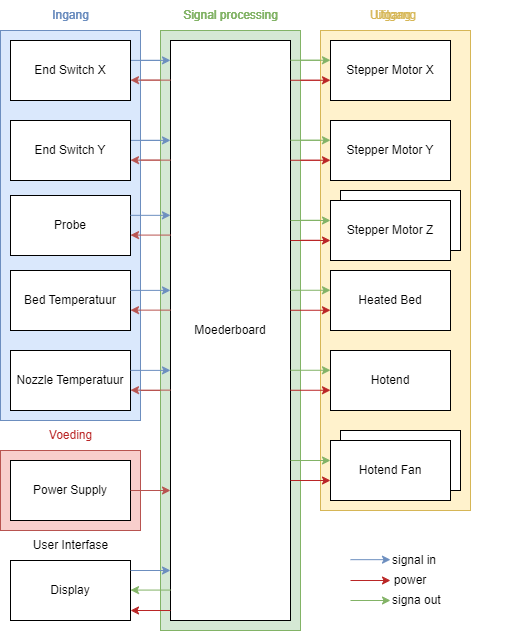
\includegraphics[width=\textwidth]{Creality Ender V2.drawio.png}
\end{figure}

\newpage
\section{FMEA}
\textbf{Scope}



\newpage
\section{Parato analyse}
\input{Parato.tex}

% \newpage
% %Bibliography
% \bibliographystyle{IEEEtran}
% \bibliography{bib}
% \addcontentsline{toc}{section}{Referenties}

% \newpage
% % Bijlage's 
% \appendix 

%   \section{Datasheet RE25 118745}
%     \label{app:datasheet motor}
%     \begin{figure}[htbp]
%       \centering % trim=left bottom right top
%       \includegraphics[page=1, clip, trim=0cm 0cm 0cm 0cm, scale = 0.65]{datasheet_RE25118745.pdf}
%       % \caption{datasheet RE25 118745}
%     \end{figure}
%     \cite{Maxon}

%   \newpage

%   \section{Datasheet GP 32 A 166158}
%     \label{app:datasheet transmissie}
%     \begin{figure}[htbp]
%       \centering % trim=left bottom right top
%       \includegraphics[page=1, clip, trim=0cm 0cm 0cm 0cm, scale = 0.65]{datasheet Planetary Gearhead GP 32 A 166158.pdf}
%       % \caption{datasheet Planetary Gearhead GP 32 A 166158}
%     \end{figure}
%     \cite{Maxon}


\end{document}